\documentclass[AMA,STIX1COL]{WileyNJD-v2}

\articletype{Article Type}%

\received{26 April 2016}
\revised{6 June 2016}
\accepted{6 June 2016}

\raggedbottom

\begin{document}

\title{Bayesian hierarchical mixture cure modelling \protect\thanks{This is an example for title footnote.}}

\author[1]{Nathan Green*}

\author[2,3]{Gianluca Baio}

\author[3]{Author Three}

\authormark{N Green \textsc{et al}}

\address[1]{\orgdiv{Department of Statistical Science}, \orgname{UCL}, \orgaddress{\state{London}, \country{UK}}}

\address[2]{\orgdiv{Org Division}, \orgname{Org Name}, \orgaddress{\state{State name}, \country{Country name}}}

\address[3]{\orgdiv{Org Division}, \orgname{Org Name}, \orgaddress{\state{State name}, \country{Country name}}}

\corres{*Nathan Green \email{n.green@ucl.ac.uk}}

\presentaddress{}

\abstract[Summary]{This paper is concerned with the ...}

\keywords{Bayesian, survival analysis}

\jnlcitation{\cname{%
\author{Green N.}, and
\author{G. Baio}} (\cyear{2021}), 
\ctitle{}, \cvol{2017;00:1--6}.}

\maketitle

\footnotetext{\textbf{Abbreviations:} MCM, mixture cure model; APC, antigen-presenting cells}


\section{Introduction}\label{sec:intro}

{\it set the scene}\\
better diagnosis and screening has lead to more cured cancer patients.
Note that 'cured' means has a general population mortality rate.
Cure models split patients in to two (or more?) groups: cured or not.
Individual are subject to one to two source of risk.
There are several types of cure models.
(see \cite{Yu2013} for a comparison and guidance with application to oncology.)


Immuno-oncologic (IO) studies for melanoma therapies, such as ipilimumab, nivolumab, and the nivolumab + ipilimumab combination, have indicated that survival curves "plateau" (a considerable proportion of patients are "long-term survivors"). Cure models are a special type of survival analysis where this "cure fraction" (the underlying proportion of responders to treatment/long-term survivors) is accounted for. Cure models estimate the cure fraction, in addition to a parametric survival function for patients that are not cured. The mortality risk in the cured patients is informed by a background mortality rate. The population that is not cured is subject both to background mortality and to additional mortality from their cancer, estimated using a parametric survival model.
\cite{Amico2018}

Why are MCM important, specifically in health economics?
more prevalent in HEA
plateau in events

Brief review of existing applications


BMC to give background...

limitations?
Q. can we do better?
i) PFS from OS
ii) pooled fraction

Our innovative proposal:
In this paper...joint model of PFS and OS, which has the double advantage of borrowing information
(eg the likely more mature PFS data to inform the highly censored OS)
*and* obtaining a pooled cure rate.

We will take a Bayesian approach; for a non-cure fraction model survival analysis in health economics \cite{Demiris2006,Jackson2010}.

% software
This analysis has been carried-out using the Stan inference engine
\cite{carpenter2017stan} called from R on a Windows PC.
The details of the algorithm can be found in the Appendix.
The packaged code can be downloaded from here.


\section{Motivating example}\label{sec:example}
Our motivating example concerns
long term
different cut points

\subsection{BMS data}
The data source for the analysis is the patient-level data from the CheckMate 067 trial [ref?].
Our dataset contains $n = 945$ subjects (8 with a missing treatment indicator, i.e. the actual treatment received). The treatment groups are as  follows:
\begin{description}
\item[Nivolumab monotherapy] 3 mg/kg intravenous (IV) once every 2 weeks (Q2W). 313 patients were treated (203 PFS events and 175 OS events). Median PFS and OS are 6.93 months (95\% confidence interval (CI) 5.32 - 10.41) and 36.9 months (95\% CI 31.24 - 60.9), respectively. {\it should time be in months/days?}
\item[Ipilimumab monotherapy] 3 mg/kg IV once every 3 weeks (Q3W) for a total of 4 doses. 311 patients have been treated (261 PFS events and 228 OS events). Median PFS and OS are 2.86 months (95\% CI 2.79 - 3.29) and 20.0 months (95\% CI 17.22 - 25.6), respectively.
\item[Combined nivolumab with ipilimumab] 1 mg/kg IV and 3 mg/kg IV Q3W for 4 doses followed by nivolumab 3 mg/kg IV Q2W. 313 patients were treated (182 PFS events and 151 OS events). Median PFS is 11.50 months (95\% CI 9.26 - 20.80) and median OS not reached. 
\end{description}


{\it How it compares with dataset prevalent in our field/applications? BMS?}


\section{Methods}\label{sec:methods}

\begin{figure}
\centering
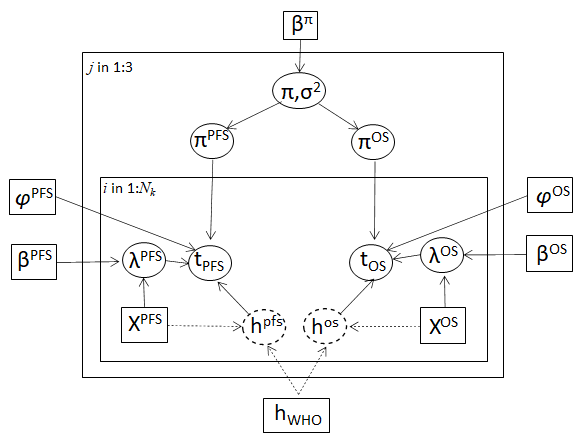
\includegraphics[width=0.6\linewidth]{DAG_with_Tx.png}
\caption{\label{fig:hier_dag} Hierarchical cure fraction DAG for PFS and .}
\end{figure}

\subsection{The standard mixture cure model} \label{section:basic_model}
{\it Description of "standard" model and the frequentist approach typically used}\\
The standard mixture cure model (MCM), which is the basic of the proposed model, is a type of cure model where survival is modelled as a mixture of two groups of patients: those who are cured (and so will never experience the event of interest) and those who are not (and who therefore remain at risk).
The combined survival for a population with a cure fraction can be written as follows:

\begin{equation}
\label{eqn:mcm}
S(t, x) = S^*(t, x) [\pi(x) + (1 - \pi(x)) S_u(t, x)],
\end{equation}
\\
\noindent
where $S(t)$ denotes the survival at time $t$, $S^*(t, x)$ denotes the background mortality
at time $t$ conditional on covariates $x$, $\pi(x)$ denotes the probability of being
cured conditional on covariates $x$, and $S_{u}(t, x)$ denotes the mortality due to 
cancer at time $t$ conditional on covariates $x$.

\subsubsection{Likelihood}
Let $T_i$ be a non-negative event time and $C_i$ be a censoring time for the $i$th individual. Then define the censoring indicator $\delta_i = I(T_i < C_i)$ and variable denoting the observed survival time $t_i = \min(T_i, C_i)$. Either $\delta_i = 1$ or $0$ denoting an event or censored observation at $t_i$. The observed data on the $i$th individual are thus $\mathcal{O}_i = (t_i, \delta_i, \boldsymbol{x}_i),\; i = 1, \ldots, N$, where $\boldsymbol{x}_i$ is the covariate vector.
Covariates may be experimental (e.g. treatment assignment) or prognostic factors.
In the simplest case we can assume that the cure fraction is the same
for the whole population i.e. $\pi$ is fixed. Further, we can assume the
$\pi$ models the relationship between $\boldsymbol{x}_i$ and the
probability of being cured. E.g. using a logistic-linear model

$$
\pi(\boldsymbol{x}_i | \boldsymbol{\beta}) = 1/[1 + \exp(-\boldsymbol{x}_i^T \boldsymbol{\beta})].
$$
The likelihood of the standard survival is
$$
L = \prod_i S(t_i | \boldsymbol{x}_i) h(t_i | \boldsymbol{x}_i)^{\delta_i}
$$
Log-likelihood is therefore
$$
\mathnormal{l} = \sum_i \log(S(t_i | \boldsymbol{x}_i)) + \delta_i \log(h(t_i | \boldsymbol{x}_i))
$$
Plugging this directly into the mixture cure equation in (\ref{eqn:mcm}) gives
$$
\mathnormal{l}(\pi | \boldsymbol{\delta}, \boldsymbol{x}) =
 \sum_i \log(S^*(t_i | \boldsymbol{x}_i) h^*(t_i | \boldsymbol{x}_i)^{\delta_i}[\pi(x) +
   (1 - \pi(x)) S_u(t_i | \boldsymbol{x}_i) h_u(t_i | \boldsymbol{x}_i)^{\delta_i}])
$$
If we assume that the cured component is the Exponential survival model
then the non-cured component can be thought of in similar terms to the
cumulative incidence function. That is, the probability of an event is
the combined probability of surviving both events (e.g. for OS,
all-cause and cancer mortality) and then experiencing either i.e.
dropping the $S$ dependencies for brevity

\begin{equation}
\label{eqn:surv_pdf_exp}
S^* S_u (h^*)^{\delta} + S^* S_u (h_u)^{\delta} = S^* S_u (h^* + h_u)^{\delta}
\end{equation}

\subsubsection{Bayesian inference}
Using the likelihood function defined above and prior distributions on
uncertain parameters, we can specify the posterior distribution.
Defining $g_2$ as the prior distribution for the coefficients of the
uncured fraction $\beta^u$ and $g_3$ as the prior distribution for the
coefficients of the cured fraction $\beta^*$, then the general form of
the posterior distribution can be written as follows.

\begin{equation}
\label{eqn:basic_posterior}
p(\pi, \boldsymbol{\beta^u}, \boldsymbol{\beta^*} | \mathcal{O}) \propto
L(\pi, \boldsymbol{\beta^u}, \boldsymbol{\beta^*} | \mathcal{O}) f(\pi) g_2(\boldsymbol{\beta^u}) g_3(\boldsymbol{\beta^*})
\end{equation}
assuming that the cure fraction is independent of the covariates.

\subsection{The hierarchical mixture cure model}
Extending the notation of Section~\ref{section:basic_model}, denote the observed data on the $i$th individual for two survival event types as $(t_{1i}, t_{2i}, \delta_{1i}, \delta_{2i}, \boldsymbol{x}_i),\; i = 1, \ldots, N$.
From now on we will assume that these two event types are progression-free survival and overall survival.
Covariates can be different for PFS, OS and $\pi$ but we shall use $x$ throughout for simplicity.

A multilevel frailty cure fraction model for the latent variable formulation was considered by \cite{Tawiah2020}.

A related generalisation by \cite{Balogun2020} consider a single event type but multiple co-infections with different cure fractions, similar to how we have different cure fractions for each treatment.

\subsubsection{Bayesian inference}
From (\ref{eqn:basic_posterior}) we can extend the formulation as follows

$$
p(\pi, \boldsymbol{\beta^{OS}}, \boldsymbol{\beta^{PFS}}, \boldsymbol{\beta^*} | \mathcal{O}_{OS}, \mathcal{O}_{PFS}) \propto
L(\pi, \boldsymbol{\beta^{OS}}, \boldsymbol{\beta^*} | \mathcal{O}_{OS}) L(\pi, \boldsymbol{\beta^{PFS}}, \boldsymbol{\beta^*} | \mathcal{O}_{PFS}) f(\pi) g_{OS}(\boldsymbol{\beta^{OS}}) g_{PFS}(\boldsymbol{\beta^{PFS}}) g(\boldsymbol{\beta^*})
$$
\\
\noindent
The (cure subpopulation) incidence model for each individual is expressed in terms of a fixed-effects logistic regression

$$
\text{logit}(\pi) = \beta^{\pi}_1 + \beta^{\pi}_2 TRT,
$$
where $\beta^{\pi}_1$ represents an intercept and $\beta^{\pi}_2$ is the regression coefficient for the $TRT$ covariate.
Note that we could also include a frailty term for individual $i$.

\subsubsection{Cure fraction}
There are two obvious ways to represent the uncertainty about the cure
fraction in the model.

The first is to specify the cure fraction directly using a
$\pi \sim \text{Beta}(a_{cf}, b_{cf})$ prior, most uninformative as a uniform
$\text{Beta}(1,1)$. The parameters can be obtained via transformation of mean
and standard deviation to allow a more natural scale for elicitation.

Alternatively, we may specify the uncertainty on the real line with a
Normal distribution and then transform to the probability scale.
A further consideration is how to represent the cure fraction so to
share information between the OS and PFS data. We will investigate 3
alternatives.

\begin{description}
    \item[Pooled] Assume that the cure fraction is the same for OS and PFS
    i.e. $\pi_{os} = \pi_{os} = \pi$ where $$
    \text{logit}(\pi) \sim \text{N}(\mu_{cf}, \sigma_{cf}^2), \;\;
    $$
    \item[Separate] Model each independently. $$
    \text{logit}(\pi_{os}) \sim \text{N}(\mu_{cfos}, \sigma_{cfos}^2), \;\;  
    \text{logit}(\pi_{pfs}) \sim \text{N}(\mu_{cfpfs}, \sigma_{cfpfs}^2)  
    $$
    \item[Hierarchical] Assume exchangeability between OS and PFS$$
    \pi \sim \text{N}(\mu_{cf}, \sigma_{cf}^2), \;\;  
    \text{logit}(\pi_{os}) \sim \text{N}(\pi, \sigma_{cfos}^2), \;\;  
    \text{logit}(\pi_{pfs}) \sim \text{N}(\pi, \sigma_{cfpfs}^2)  
    $$
\end{description}

\subsubsection{Background survival}
We used the World Health Organization
(WHO) life tables by country for the latest year available of 2016
\cite{wholifetables} to inform the background mortality rate (baseline
hazard). These baseline hazards are the expected mortality rate for each
patient at the age at which they experience the event. The mortality
data are age- and gender adjusted, thus providing a granular account of
the different patient profiles in the trial. The WHO reports conditional
probabilities of death in 5-year intervals until age 85. A constant
annual mortality rate is reported for individuals over 85. They assumed
that the maximum age is 100 years.

In a Bayesian analysis there are alternative ways in which we could
model the background mortality.

For this work we shall use WHO hazard point estimates as known. We could
consider the WHO estimates to provide sufficiently accurate estimates
given the sample size and so incorporating uncertainty is not necessary.
This also forces consistency across fits. Denote the WHO estimates for
individual $i$ as $\hat{f}_i, \hat{S}_i, \hat{h}_i$ for the density,
survival and hazard respectively.

This gives the likelihood
$$
L(\pi | \boldsymbol{\delta}, \boldsymbol{x}, \hat{S}, \hat{h}) =
\sum_i \hat{S}_i \hat{h}_i^{\delta_i} \left[ \pi(x) + (1 - \pi(x)) S_{u, i} h_{u , i}^{\delta_i} \right]
$$

{\it Sharples ref re Gamma process?}

{\it implications?}

\subsubsection{Prior specification}
The choice of priors should be informed by expert opinion.
We specify vague priors on log-scale for the coefficients of the OS and PFS rates. Centering the ages, the baseline is $\beta_0^{PFS} \sim \text{Normal}(0, 100),\; \beta_0^{OS} \sim \text{Normal}(0, 100)$ and for age $\beta_{age}^{PFS} \sim \text{Normal}(0, 100),\; \beta_{age}^{OS} \sim \text{Normal}(0, 100)$.
This corresponds to median survival time of xxx.
We don't wish to apply covariate effect to the other parameters of the OS and PFS time distributions so we specify the priors directly on the parameter e.g for the Weibull distribution shape parameter $\nu \sim \text{Gamma}(2, 2)$. 
The level-one cure fraction is modelled as a fixed effect linear regression with logistic link and coefficient priors $\alpha \sim \text{Normal}(0, 100)$.
The level-two cure fraction distribution for OS and PFS have logistic-normal priors for the probabilities with variances $\sigma^2_{PFS} \sim \text{Gamma}(2, 2),\; \sigma^2_{OS} \sim \text{Gamma}(2, 2)$.



\section{Application}\label{sec:application}

Back to BMS data and results, with various scenarios/distributions and all the plots and tables, similar to the ones Nathan has already provided

\subsection{PFS and OS modelled separately}
\subsection{Exchangeable cure fraction}
\subsubsection{Treatments modelled separately}
\subsubsection{Treatments modelled jointly}

Exponential, Weibull, Gompertz, Log-Normal, Log-Logistic\\
{\it model assessment?}



\section{Discussion}\label{sec:discussion}



%\backmatter

\section*{Acknowledgements}
This is acknowledgement text.

\subsection*{Author contributions}

This is an author contribution text.

\subsection*{Financial disclosure}

None reported.

\subsection*{Conflict of interest}

The authors declare no potential conflict of interests.


% \section*{Supporting information}

% The following supporting information is available as part of the online article:

% \noindent
% \textbf{Figure S1.}
% {500{\uns}hPa geopotential anomalies for GC2C calculated against the ERA Interim reanalysis. The period is 1989--2008.}


% \appendix

% \section{Section title of first appendix\label{app1}}

% with normal text font. Refer below example:

% \begin{lstlisting}[caption={Descriptive Caption Text},label=DescriptiveLabel]
% for i:=maxint to 0 do
% \end{lstlisting}

% %\nocite{*}% Show all bib entries - both cited and uncited; comment this line to view only cited bib entries;
\bibliography{bibliography}

% \clearpage

% \section*{Author Biography}

% \begin{biography}{
\includegraphics[width=66pt,height=86pt,draft]{empty}}{\textbf{Author Name.} This is sample author is sample author biography text.}
% \end{biography}

\end{document}
